\documentclass
	[ a4paper	% paper format
	, 10pt		% fontsize
	, twoside	% double-sided
	, openright	% begin new chapter on right side
	, notitlepage	% use no standard title page
	, parskip=half	% set paragraph skip to half of a line
	]{scrreprt}

\usepackage[english]{babel}
\usepackage{amsmath}
\usepackage{latexsym}
\usepackage[T1]{fontenc}
\usepackage[utf8x]{inputenc}
\usepackage{graphicx}
\usepackage[hidelinks]{hyperref}	% "hidelinks" removes the border around links
\usepackage{tabularx}
\usepackage{color}			% Colors
\usepackage{colortbl}			% Table colors
\usepackage{makecell}			% Xhline
\usepackage{multirow}
%\usepackage{etoolbox}
\usepackage{amsfonts}
\usepackage{fancyhdr}
\usepackage{amsthm}
\usepackage{amssymb}			% \blacklozenge
\usepackage{lscape}
\usepackage{hhline}
\usepackage{multicol}
\usepackage{lastpage}
\usepackage{mathtools}
\usepackage{tcolorbox}
\usepackage{minted}
\usepackage{geometry}
\usepackage[english]{babel}
\usepackage{fancyhdr}
\usepackage{parskip}
\geometry{
	a4paper,
	total	= {170mm, 257mm},
	left	= 20mm,
	top	= 30mm,
	bottom	= 30mm
}

% Header and footer
% The use of "\chapter" forces "\pagestyle{plain}", therefore both page styles
% "plain" and "fancy" have to be set
\newcommand{\mystyle}{
	\fancyhf{}
	\lhead{Bern University of Applied Sciences}
	\rhead{CHVote Demonstrator}
	\lfoot{}
	\cfoot{Page \thepage\ of \pageref{LastPage}}
	\rfoot{}
}

\pagestyle{fancy}
\mystyle
\fancypagestyle{plain}{\mystyle}

% Paragraph configuration
\setlength{\parindent}{1em}
\setlength{\parskip}{1em}

% Quotes
%\usepackage[autostyle, english = american]{csquotes}
%\MakeOuterQuote{"}

%\addto\captionsenglish{\def\figurename{Figure}}
%\addto\captionsenglish{\renewcommand{\chaptername}{Chapter}}
%\selectlanguage{english}

%\makeatletter
%\renewcommand{\@chapapp}{Chapter}
%\makeatother

%\tcbuselibrary{theorems}
%
%\theoremstyle{definition}
%\newtheorem{exmp}{Beispiel}[subsection]
%\renewcommand{\chaptername}{Chapter}
%\newmintinline['macro name']{'language'}{'options'}
%
%\newtcbtheorem[number within=section]{mytheo}{Theorem}
%{colback=green!5,colframe=green!35!black,fonttitle=\bfseries,before
%skip=20pt plus 2pt,after skip=20pt plus 2pt}{th}
%
%\makeatletter
%\def\@seccntformat#1{
%	\expandafter\ifx\csname c@#1\endcsname\c@subsection\else
%	\csname the#1\endcsname\quad
%	\fi
%}
%\makeatother


\begin{document}
%\pagestyle{empty} % hide header and footer on title page

\begin{titlepage}
\begin{center}
	
\includegraphics[width=0.08\textwidth]{assets/bfh_logo.png}

	\vspace{1cm}

	\textsc{\Large Bern University of Applied Sciences (BFH)} \\[1.5cm]
	\textsc{\Large Bachelor Thesis} \\[1cm]

	\newcommand{\HRule}{\rule{\linewidth}{0.3mm}}
	\HRule \\[0.4cm]
	{\Large \bfseries Visualizing Geneva's Next Generation E-Voting System} \\
	\HRule \\[1.5cm]

	\begin{tabular}{rl}
	\textbf{Authored by}
	& Kevin \textsc{Häni} <\href{mailto:kevin.haeni@gmail.com}{kevin.haeni@gmail.com}> \\
	& Yannick \textsc{Denzer} <\href{mailto:yannick@denzer.ch}{yannick@denzer.ch}> \\
	\textbf{Supervised by}
	& Prof. Dr. Rolf \textsc{Haenni} <\href{mailto:rolf.haenni@bfh.ch}{rolf.haenni@bfh.ch}> \\
	& Prof. Dr. Philipp \textsc{Locher} <\href{mailto:philipp.locher@bfh.ch}{philipp.locher@bfh.ch}> \\
	\end{tabular}

	\vfill

	Bern, {\large \today}
\end{center}
\end{titlepage}


\clearpage
\tableofcontents
%\listoftables
%\pagestyle{plain}

\clearpage
\chapter{Introduction}
\section{Electronic voting}
Since 2015, it is possible for Swiss citizens registered in the cantons Geneva and Neuchâtel and living abroad, to vote electronically. However, these systems did not yet meet the requirements in terms of security and transparency, to be accepted as a secure E-Voting platform on a nationwide scale.

One of the requirements that is hardest to achieve, is that the system must ensure the voters privacy while at the same time, it must be verifiable that only valid votes have been counted. A good e-voting system must be transparent and allow an external verifier to verify, that every protocol participant has abided by the protocol and that all votes of eligible voters have been counted correctly.

Another common problem is the insecure platform problem: If a voters computer is affected by malware, the vote casting process is no longer under the voters control and the candidate selection could be possibly manipulated. 

A contract was formed between the state of Geneva and the Bern University of Applied Sciences to work out a new protocol which does meet the complex requirements set up by the government. In 2017, the resulting specification document has been officially published and a proof-of-concept / prototype has been successfully implemented by the State of Geneva. 

\section{The CHVote protocol}
The protocol our project is based on, does not originate from us! The concept and specification has been created by Rolf Haenni, Philipp Locher and Reto E. Koenig of the Institute for Security in the Information Society (RISIS) of the Bern University of Applied Sciences. For this project, we have implemented the protocol according to their specification. In this section we summarize the most important aspects of the protocol for better understanding our application.

\subsection{Actors}
\textbf{Voter: } A voter is a person who is eligible to vote in his state. Every voter must possess a voting card that has been sent to him prior to an election and that contains several codes such as the voting code and the confirmation code, which are used to identify the voter during the vote casting process.

A voter uses a voting client to participate in the protocol, e.g. forming a ballot according to the protocol, by entering his selection, a voting code to cast, and later in the process, his confirmation code to confirm his vote. Verification codes and a finalization code are displayed by the voting client to ensure the voter that his vote has been cast as intended and hasn't been manipulated by a third party.

\textbf{Election Administrator}: The election administrator, typically a person of the government, sets up the election by providing the necessary information such as the candidates and the voters and initiates the generation of the cryptographic electorate data. He is also responsible for tallying the election and publishing the final results.

\textbf{Election Authorities}
The election authorities can be seen as some kind of independent election observers. In a CHVote election there are always multiple election authorities in order to avoid having a single authority that has to be trusted. The authorities are involved in almost every step of the protocol, starting from generating their shares of the electorate data, shares of a joint public key used for encryption, checking and responding to new ballots and vote confirmations, as well as in the mixing and decryption phases.

\textbf{Bulletin Board}
The bulletin board acts as a central board over which most communication is done and where all the public data is stored.

\textbf{Printing Authority}
The printing authority is responsible for printing the voting cards and handling them over to a trusted mailing service. Since the printing authority needs to print the voting cards that contain the sensitive voting and confirmation code, it is the only participant possessing the secret voting codes of all voters.  

\subsection{Pre-Election \& Voting cards}
Before the actual election phase, the vote administrator sets up the election by entering all required parameters. All election authorities jointly generate the cryptographic data for the whole electorate from which the voting card information is derived. The printing authority combines the information from all election authorities, prints the voting cards and deliver them to the voters by a trusted mailing service. 

A voting card contains several codes, namely:

\begin{itemize}
	\item a voting code
	\item a confirmation code
	\item a finalization code
	\item one verification code for every candidate
\end{itemize}

The voting and confirmation codes are authentication codes and used to authenticate the voter twice during the vote casting process; the first time with the voting code when he casts his vote, and a second time for confirming his vote. A second authentication code is required because otherwise an attacker who infected a voters computer with malware could just confirm a vote on behalf of the voter after he manipulated the candidate selection. 

\subsection{Cast-as-intended verification with oblivious transfer}

Even with the authentication codes, an insecure voting platform infected with malware still poses the risk that an attacker manipulates the candidate selection on the vote-casting page after the voter has entered his voting code. 

The CHVote specification suggests a "`Cast-as-intended verification"' to allow voters to detect this kind of manipulation:

When a voter enters his voting code and the indices of his favored candidates, the voting client forms a \textbf{ballot} containing the voters selection encrypted with the authorities public key, his public voting credential derived from the voting code, and a zero knowledge proof which proofs that the voter has formed the ballot according to the protocol and that he has been in knowledge of his voting code.

Every election authority now checks the voters public voting credential, the validity of the ballot proof and that the voter hasn't already cast a vote. 

The encrypted selection also serves as a query for an oblivious transfer. A k-out-of-n oblivious transfer allows a client to query a server for k messages, without the server knowing what k messages the client requested, and without the client learning anything about the n-k other messages. Adapted to the CHVote protocol, the query queries the authorities for the corresponding verification codes of the selected candidates, without the authorities learning which candidates the voter has selected, and without revealing any information about the other candidates. 

The voter then checks if the returned verification codes match the codes of the candidates he has chosen on the printed voting card. If the selection was somehow manipulated by malware, the returned verification codes would not match the printed ones and the voter would have to abort the vote casting process. This way the integrity of the vote casting can be assured even in the presence of malware. In such a case, privacy on the other hand cannot be protected since the malware will learn the plaintext of the voter's selection.

In order to verify that a voter has formed the ballot correctly by choosing exactly the number of candidates he is supposed to choose, the following trick is being used: the verification codes are derived from $n = \sum_{n=1}^{t} n_j$ random points on $t$ polynomials (one for every election event $j$) of degree $k_j - 1$, that each election authority has chosen randomly prior to the election. By learning exactly $k = \sum_{n=1}^{t} k_j$ points on these polynomials, the voting client is able to reproduce these polynomials and therefore is able to calculate a particular point with $x=0$ on these polynomials. The corresponding $y$ values are incorporated into the second voting credential from which the confirmation code is derived. Only if the voter knows these points (by submitting a valid candidate selection), he will be able to confirm the vote that he casted.

\subsection{Re-encryption mix network}

Since there is still a connection between the encrypted ballot and the voter at this point, the encrypted selections are extracted from the ballots as the first step of the post-election phase. In order to anonymize the list of encryptions, every authority performs a cryptographic shuffle with a random permutation and re-encrypts all ciphertexts in order to make it impossible to find out which voter has submitted which encrypted ballot. This is done by using the multiplicative homomorphic property of the ElGamal encryption scheme. A multiplicative homomorphic encryption scheme allows to perform multiplications on the ciphertext such that:

\begin{equation*}Enc(a) \cdot Enc(b) = Enc(a \cdot b)\end{equation*}

The specification suggests multiplying the encryption with the encryption of the neutral element $1$ since this yields a new ciphertext for the exact same plaintext.

\subsection{Distributed trust}
The public key that is used for encrypting the ballots has been jointly generated by all election authorities. Therefore in order to decrypt the result, all authorities must provide their share of the private key. The measure of multiple authorities participating in the whole e-voting process ensures the security of the whole election even if only one authority can be trusted.

\section{Project task}

Understanding such a complex protocol isn't easy and might be the reason why many people still do not trust electronic e-voting systems. In close consultation with the authors of the CHVote specification, we agreed to develop an application that allows users to get a hands-on experience with the CHVote e-voting system and makes it possible to show to an audience how the future of voting in Switzerland might possibly look like.

For this reason, we have implemented the protocol according to the specification and developed a web-based application on top of it, which allows to perform every step of an election, from generating the electorate data, to casting and confirming ballots from a voters point of view, to the post-election processes like mixing, decryption and tallying.

\chapter*{Management Summary}

\chapter{Technical Implementation}
In this chapter, we will describe how we implemented our application. We will start explaining the architecture from a high-level perspective with each component being a black-box. Later sections of this chapter will then further describe the internals of every component.

We have implemented our application following a "`single page application (SPA)"' architecture. Some reasons that lead to this decision:
\begin{itemize}
	\item Due to our personal interest in JavaScript and our intention of improving our knowledge in this language, we wanted a significant part of the development to be done client-side.
	\item We imagined the state handling to be easier with a SPA than having to pass around cookies and session data between every request.
	\item A SPA seemed great for building modern looking, intuitive and responsive user interfaces.
\end{itemize}

From a high level perspective and following the SPA architecture, we have structured our application into 3 main components, as shown in figure \ref{System components}:

\begin{figure}[h!]
\begin{center}
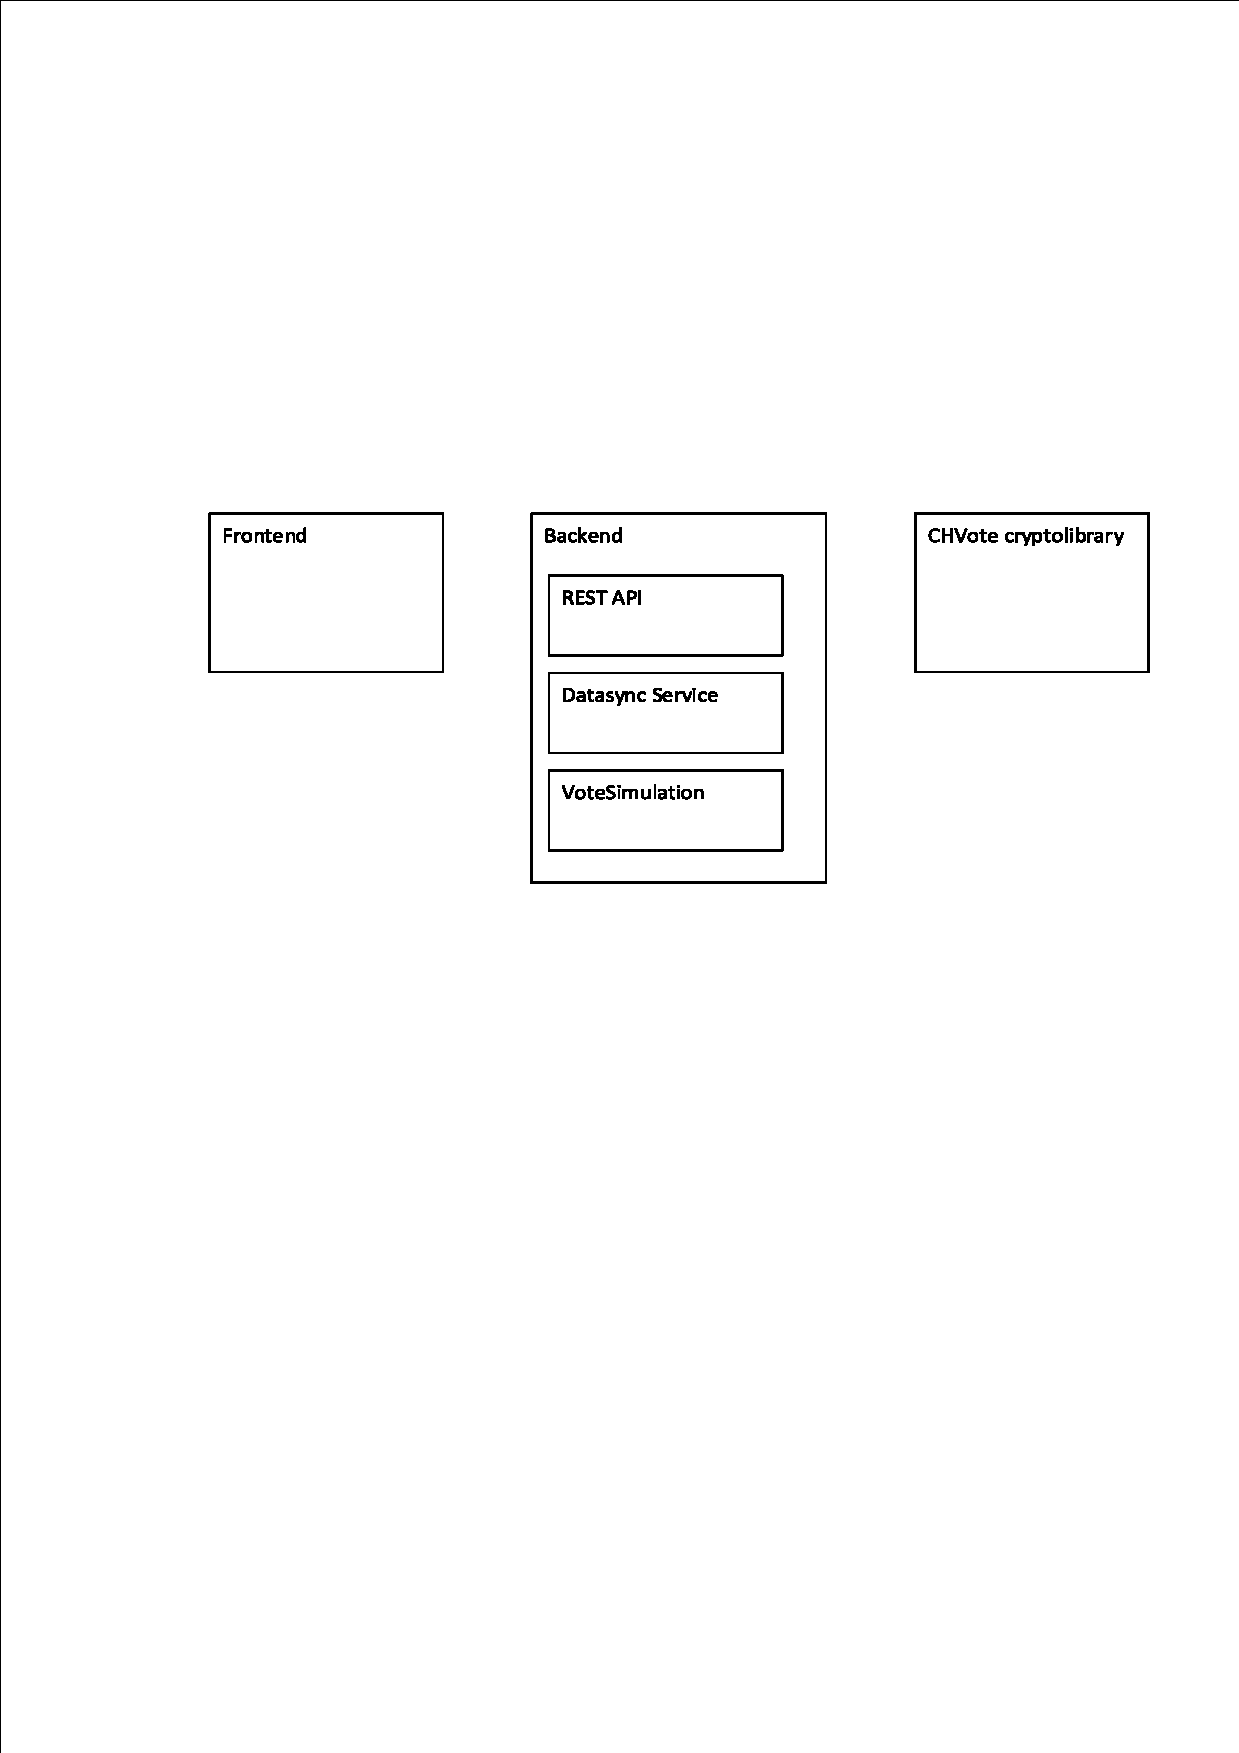
\includegraphics[scale=0.95]{assets/componentdiagram.pdf}
\captionof{figure}{From a high level perspective, our application consists of 3 main components: The front-end (web-application), the back-end, and the crypto-library.}
\label{System components}
\end{center}
\end{figure}

\begin{itemize}
	\item The \textbf{front-end} / web-application is where all the functionality of our back-end is consumed and where a typical CHVote election event is visualized for the users. It is therefore the most important component of our application. The backend is developed in response to what is needed by the frontend.
	\item The \textbf{back-end} consists of several components that make use of the CHVote crypto-library to build an actual e-voting ecosystem and providing an API to manipulate the data as well as a data-synchronization service to push data from the back-end to the web-clients. All the sub-components of the backend run on a single server.
	\item The \textbf{CHVote crypto-library} is the result of our "`Project 2"' course project which we have finished before our bachelor thesis. This library contains all the algorithms that are specified as pseudocode in the specification document.
\end{itemize}

\section{Technology \& Language Decisions}
When we implemented the CHVote crypto-library, we had evaluated and decided to use Python. Since Java has already been used by the team in Geneva, we wanted to use a different language as it was also desirable to prove that the CHVote specification can be implemented regardless of the programming language. Python seemed like a rather suitable language for our project due to the following reasons:
\begin{itemize}
	\item python is a mature language with lots of libraries
	\item python allows programs to be written in a compact and readable style, for example by supporting tuples
	\item as the protocol was not completely specified at that point and has still been undergoing some changes, we wanted to use a language in which we can adapt changes quickly and easily
	\item native support for large integers (\textit{BigInts}) and bindings for the GMP\footnote{GMP is a free library for arbitrary precision arithmetic, operating on signed integers, rational numbers, and floating-point numbers, see \url{https://gmplib.org/}.} library
	\item supports a lot of platforms
	\item many popular web development frameworks are available
\end{itemize}

Throughout the project not all of the reasons above turned out to be true or ideal. The drawbacks that we have experienced during the implementation of this project will be discussed in section \ref{ssec:PythonIssues}.

Since we used the crypto-library in our back-end, Python was also the obvious language for the whole back-end. Python offers a wide variety of frameworks for building web-services. Since we planed on building a single-page-application for the client, we chose the lightweight micro-framework flask for building a restful web-service and the data synchronization service.

For our \textbf{front-end} (web application) we evaluated several single-page application frameworks. VueJS is a new, modern and lightweight SPA framework that in contrast to Angular has a much flatter learning curve but still offered all the functionality that we needed. The VueJS add-on Vuex enabled us to establish a data-store pattern in our front-end, which makes it possible to have a copy of the back-end data-store in our web application which is synchronized in real-time through web-sockets.

\textbf{Socket.io} simplifies the usage of web-sockets and offers fallback technologies such as long-polling in case web-socket is not supported by either the browser or the web-server. Both Flask as well as VueJS have plug-ins that support and integrate socket.io.

For persisting the state of an election, we decided to use mongoDB. The reason behind this choice will be described in more detail later on.

\section{Architecture}
The core of our application is the VoteService component in our back-end which implements the e-voting protocol by utilizing all algorithms of the CHVote crypto-library according to the CHVote specification. The VoteService component internally holds the state of a whole CHVote election event and exposes functions to manipulate this state at a granularity required by our web application to implement all use cases. For example: The VoteService contains a list of ballots and exposes functions to cast a new ballot, which will generate a new ballot according to the protocol, by calling the CHVote crypto-library, and adds the ballot to the list.

On top of the VoteService we have implemented a REST service that acts a facade to the VoteService component and makes its functionality available as an API to our web-clients. The REST service also has to initialize the VoteService by loading and persisting its state from and to the database between each API call, since each API call is stateless.

One of the requirements is that all clients must be informed in real-time about mutations of the election state made by other participants. To achieve this, we have implemented a data sync service which allows to push the state of an election event to the web-clients by using the WebSocket protocol. This service is triggered by the REST service after every API call to push the delta between the old and the new state to the clients.

To establish a proper separation of concerns, the state of the VoteService is always sent to the client via the data sync service. The REST API only returns success or error codes or information that is required in response to some particular API call, and never state objects. On the other hand, the data sync service does never manipulate the state of the VoteService and is solely responsible for data synchronization.

\begin{figure}[h!]
\begin{center}
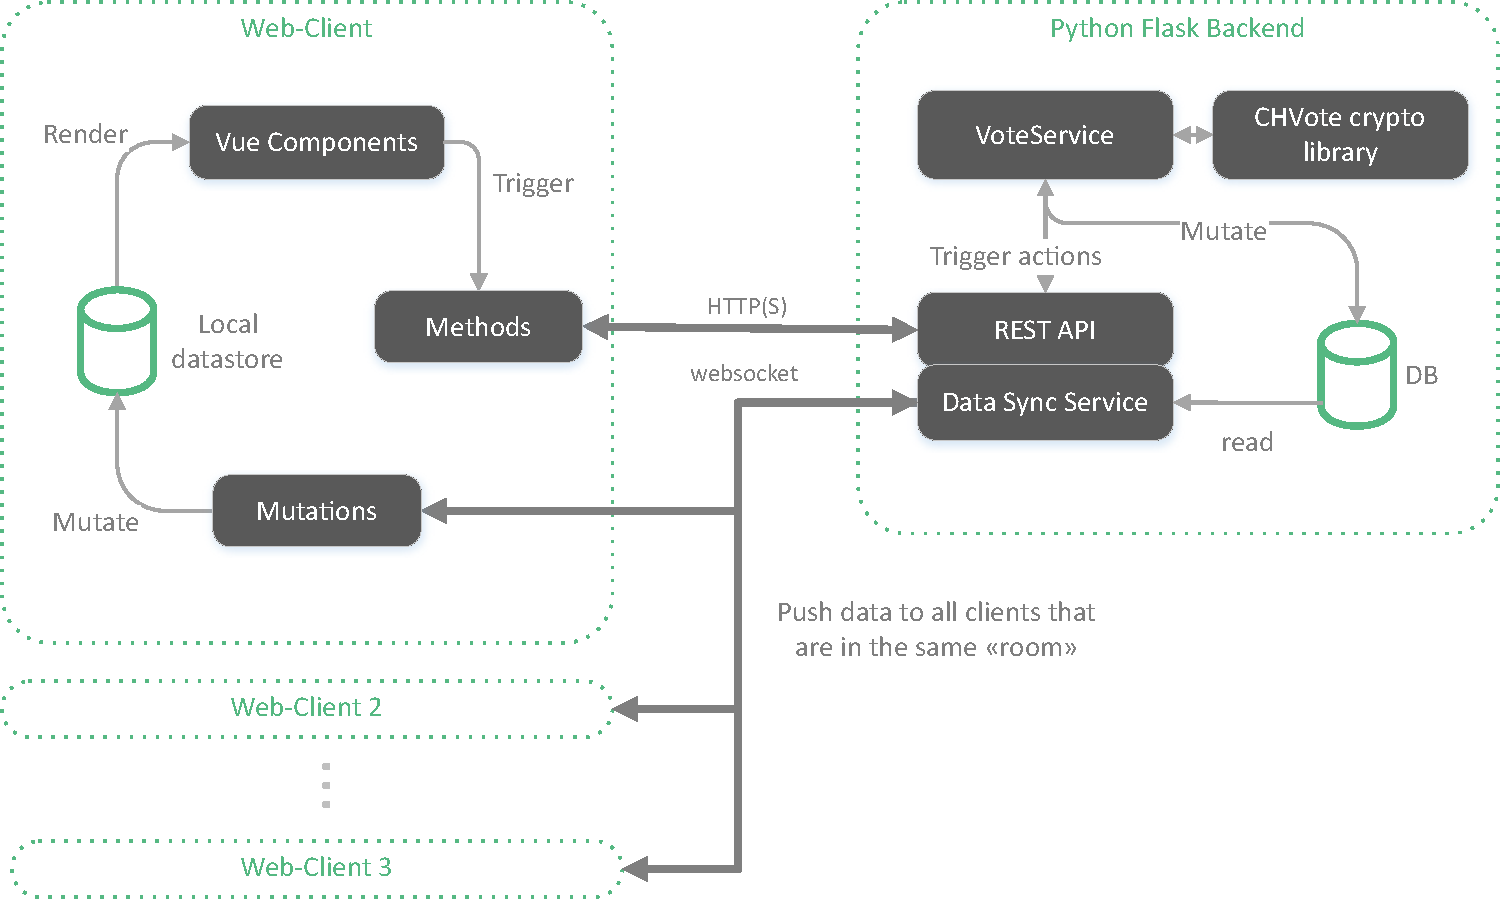
\includegraphics[scale=0.7]{assets/chvoteArchitecture.pdf}
\captionof{figure}{Our architecture with the front- and the back-end. Both sides contain a data base /data store that stores the current state of an election event. Whenever some action is called on the server side by calling our REST API, the changes are written to the database and synchronized to all clients over web-sockets. The resulting manipulations on the local datastore are automatically reflected to the user by binding the user controls to the local datastore.}\label{Architecture}%
\end{center}
\end{figure}

From the clients point of view, the web-client contains a copy of the whole VoteService state in a local data-store. This store is initially populated when the user selects an election event. Whenever the state of this election event changes, the data sync service pushes the new data to the web-client. A local mutation handler within the web application handles those messages and writes the new data into the local data-store.

Since the components that the pages of the web application are built of, are bound to the local data-store, all mutations are automatically reflected to the user. From those pages, the REST API can again be called, for example to cast a new ballot. The resulting state change is again being pushed to all clients. The responsible client that performed the API request will additionally receive a success code, or an error message in case of an error over HTTPS.

The architecture with all corresponding components is also shown in figure \ref{Architecture}
\section{Back-End}
In this section we describe the internals of the back-end services.
\subsection{VoteService}
The VoteService builds a simplified e-voting ecosystem that provides functionality to conduct an election event by internally representing the state of a whole election event. In reality, an e-voting system based on the CHVote specification would consist of multiple separate applications/services for every participant, such as a bulletin-board service for appending data to the public board, or services for every election authority for performing their tasks. Additionally, several steps of the protocol would have to be executed on the client-side, such as the generation of a voters ballots. In our application, it was reasonable to have the protocol functionality of all these parties combined within a single service.

We have decided on this VoteService centric approach mainly because we wanted to keep the whole protocol implementation within a central component and wanted to avoid having protocol logic both in the client as well as in the back-end. As an advantage, if the protocol is undergoing any changes or if our application should be extended to support a different e-voting protocol in future, only the VoteService component (and of course its dependencies as the crypto-library) will be affected or must be replaced. It also allowed us to implement the CHVote protocol almost identically as described in the specification. Because we had access to every actors data and functions from within our VoteService, passing data from one actor to another is as simple as setting an object property to some value.

Internally, we have divided the VoteService into actors and states, as shown in figure \ref{VoteService}: One actor for every protocol participant, providing the functionality a participant is responsible for, and a corresponding state-object for every actor, representing the participants current state within a given election event.

\begin{figure}[p]
\begin{center}
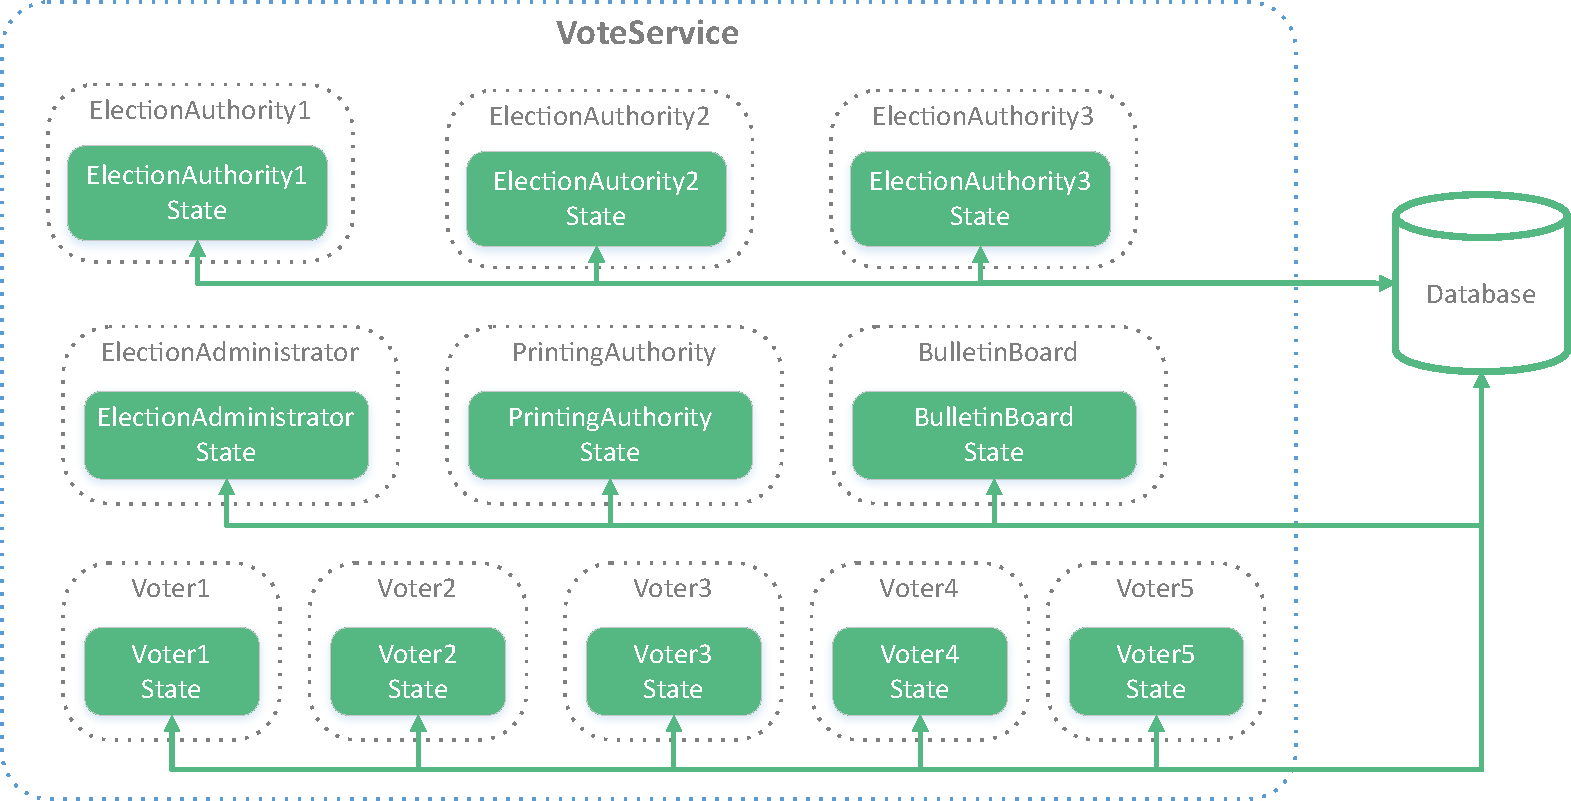
\includegraphics[scale=0.68]{assets/voteservice.pdf}
\captionof{figure}{The internals of our VoteService: The functionality is divided into actor- and state-classes. The actors provide the functionality as described in the specification and by utilizing our crypto-library. The state is contained within the state classes that allow easy serialization both for persisting them to the database as well as to a JSON representation for the data synchronization. }\label{VoteService}%
\end{center}
\end{figure}

The distinction between the actors and their states allowed us to easily serialize the state objects to JSON (a format that can be easily interpreted by the front-end) and made it easy to load and persist the state from and to the database. This measure was also necessary because of the way how we implemented our data synchronization between the clients and the back-end: By comparing and determining the differences between the state object before and after some VoteService actions, we can automatically find out the mutations that have been done to the state objects using the JSON Patch standard and generate operations to patch the clients local data store in the same way. More about this technology can be found in the section \ref{Data-Sync Service}

The only common functionality between every state object, is the ability to serialize the object to a JSON string. For this reason we had to write a custom transformer which tells the JSON parser how to serialize data-types such as mpz, byte arrays and custom classes. Luckily, python offers a way to easily serialize any custom object. By calling \mintinline{python}/object.__dict__/ we can convert an object into a dictionary, as long as the transformer is able to serialize all properties of the object.

The following list shows all the state classes, figure \ref{State classes} shows an UML representation:
\begin{itemize}
	\item \textbf{BulletinBoardState}: Holds all data that is publicly available on the bulletin board (the number of candidates, the tallied result).
	\item \textbf{ElectionAuthorityState}: Holds all data that an election authority knows (e.g. the list of ballots, the secret key of an election authority).
	\item \textbf{VoterState}: Since there is no distinction made between a voter and a voting client in our application, the VoterState contains the data of both the voter (e.g. the voting card) and the data typically known to the voting client (e.g. the points returned by the oblivious transfer).
	\item \textbf{PrintingAuthorityState}: Holds the data known to the printing authority (e.g. the list of all voters private credentials and the voting cards).
	\item \textbf{ElectionAdministratorState}: Holds all data known to the election administrator.
\end{itemize}
\begin{figure}
\begin{center}
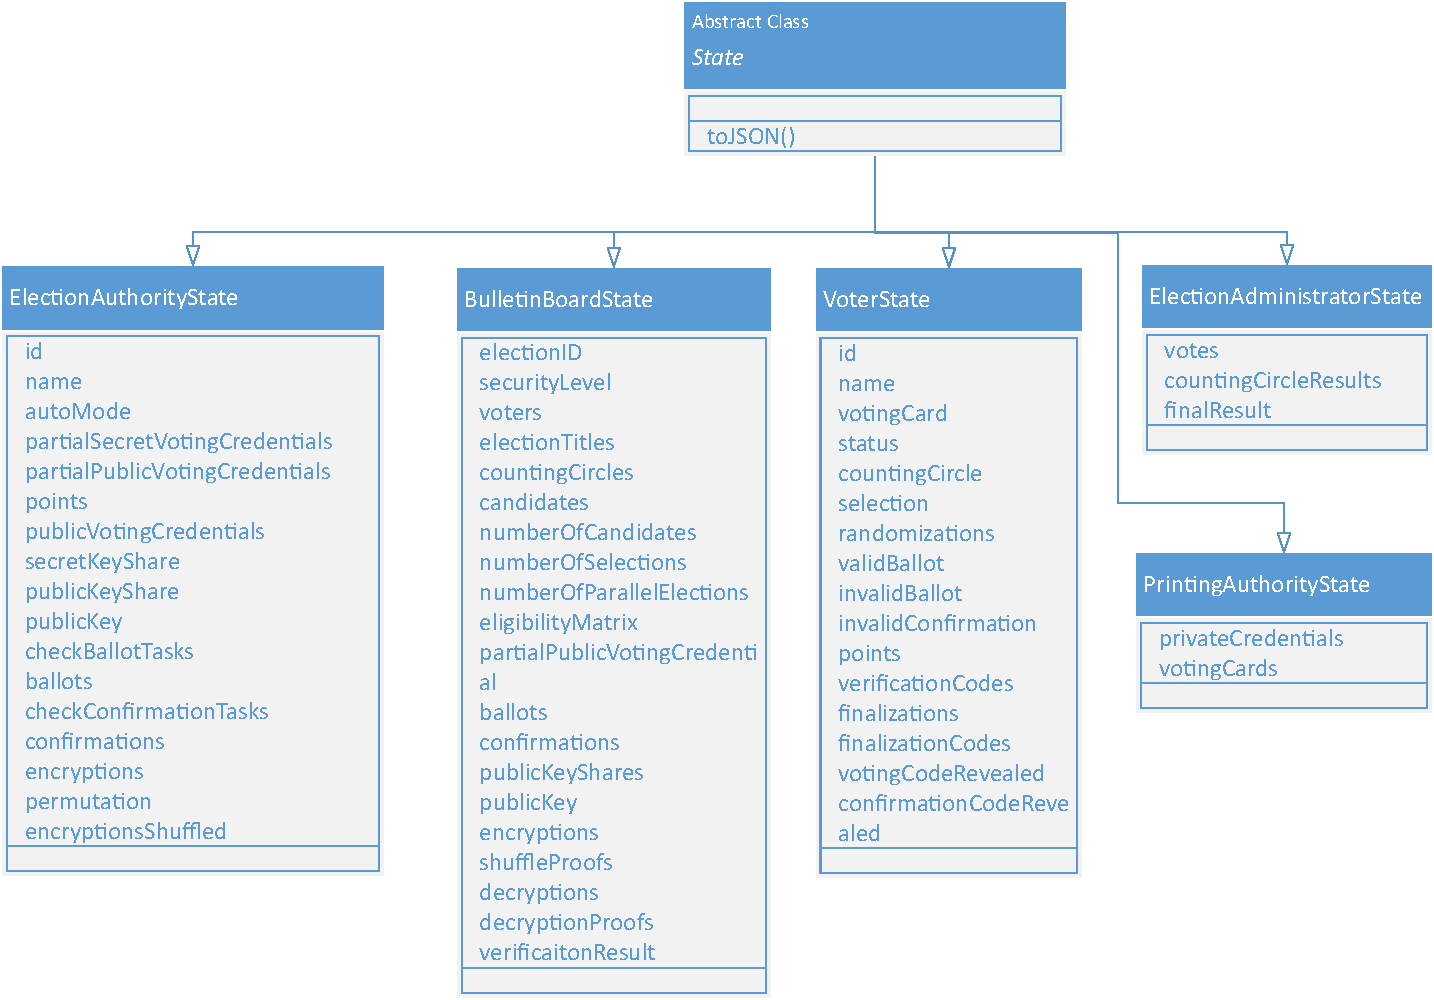
\includegraphics[scale=0.60]{assets/uml_states.pdf}
\captionof{figure}{The state of an election event is broken down into separate state classes for every participating actor. They all have in common that they are serializable to JSON}\label{State classes}%
\end{center}
\end{figure}

Since our application supports that multiple users work on different election events concurrently, the state of an election event cannot be kept in volatile memory, but needs to be persisted between every single request. For this reason we evaluated different database systems and concepts. We decided against a relational database system that requires us to define a database schema as we wanted our state objects to be the only place where the schema is defined. This "`code-first"' approach makes it easier to apply changes to the protocol in future.

For our purpose, MongoDB seemed like a good choice. Since we do not need the ability to access and filter our data by arbitrary queries, but only need to be able to save and load a state object of a particular election, we simply store the whole state as a binary string in a MongoDB collection. The only additional attribute that is saved to the database alongside with the serialized state is the electionId which denotes which election event a particular state belongs to. An election contains multiple VoterStates and ElectionAuthorityStates. Therefore, these two states additionally require an electionAuthorityId and a voterId.

\begin{figure}
\begin{center}
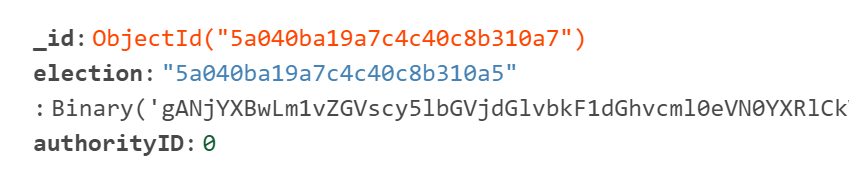
\includegraphics[scale=0.75]{assets/db.png}
\captionof{figure}{Example of a MongoDB collection (the equivalence of tables in other database systems). All states are stored as binary strings, together with an identifier for the election-event as well as the election authority ID.}\label{dbexample}%
\end{center}
\end{figure}

We described how the state classes are used to divide the data of the VoteService into smaller units. Similarly, the functionality of the VoteService is separated into classes, one for every actor of the protocol.

\begin{figure}
\begin{center}
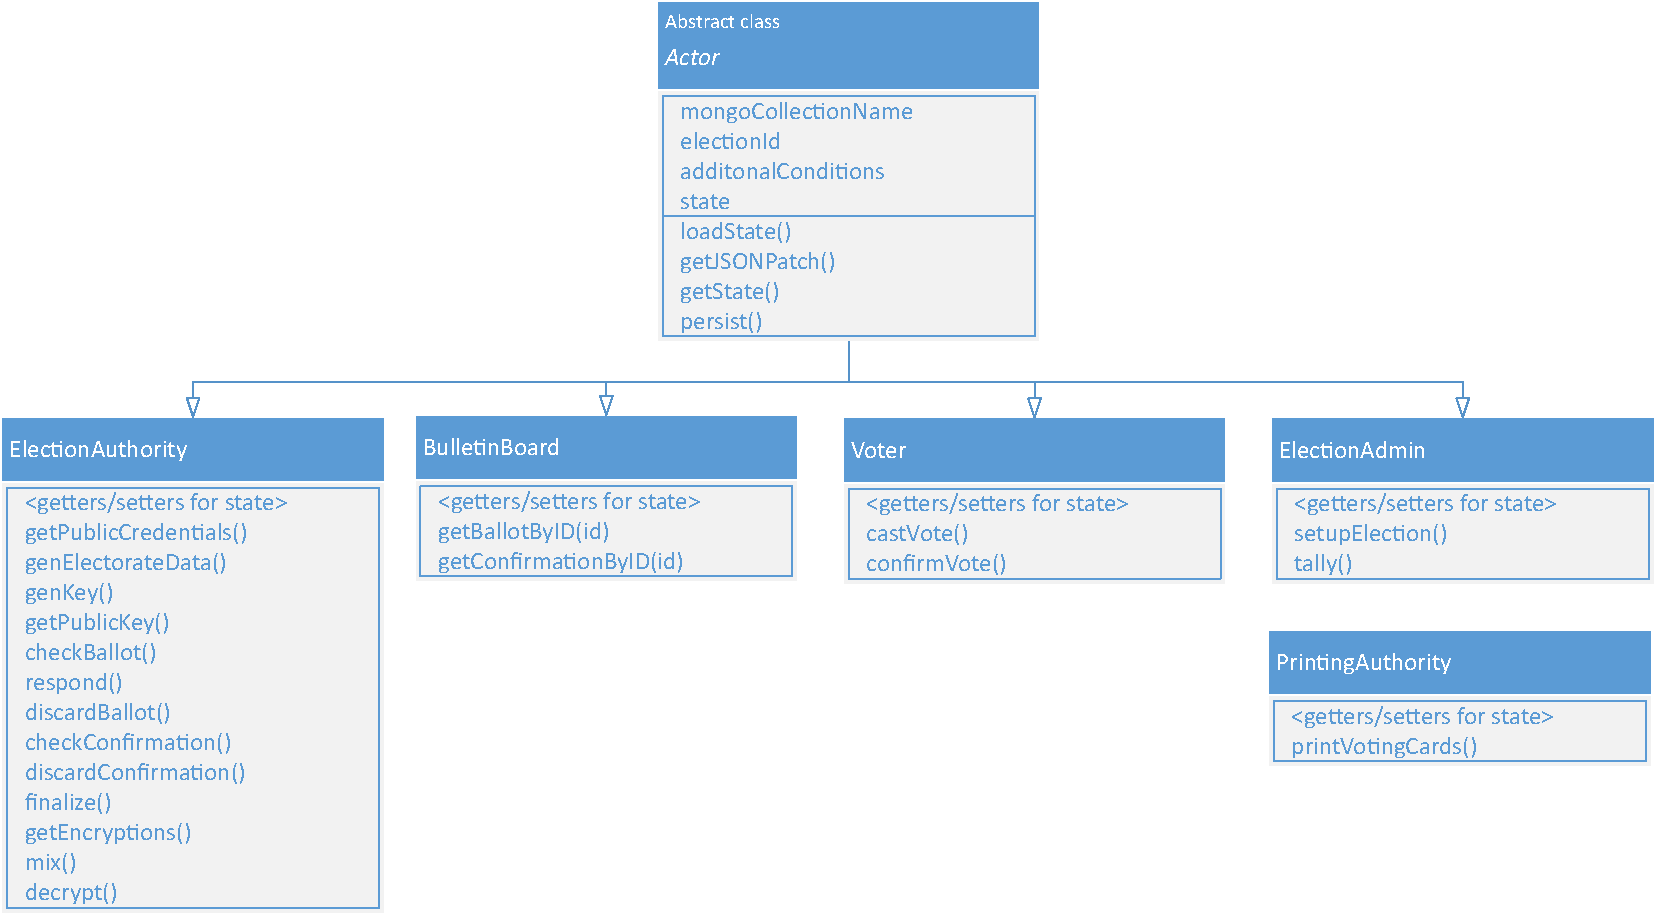
\includegraphics[scale=0.60]{assets/uml_actors.pdf}
\captionof{figure}{The functionality of the VoteService is divided into separate classes, one for every participating actor of the protocol.}\label{Actor classes}%
\end{center}
\end{figure}
The common functionality, for example functions for loading the corresponding states from the database and one for persisting the states to the database, are contained in an abstract base class.

\newpage
\subsection{Data-Sync Service}
One of the big challenges of our application has been the synchronization of an election events state between the back-end and the clients local data store. As mentioned earlier, the web-application contains a local datastore, which is structured the same way as the states of the VoteService. As per our requirements, we wanted to achieve real time data synchronization such that every web client observing a particular election event is informed of any changes of this election events state. For this purpose we have used web-sockets which - opposed to the HTTP protocol - make it possible to inform a web-client without having to rely on polling.

For the data synchronization we had to keep an eye on the performance of the data transfers since some state objects, especially the bulletin board and the election authority states grow big in size when they contain many ballots. We observed that the size of the whole state of an election event with 6 candidates and 10 voters, of which each has submitted at least one ballot and a confirmation can easily reach 600 kilobytes already. Admittedly, we have not noticed any performance issues even with rather large election events. However, transferring the whole state of an election event after every single mutation did not seem like a proper solution.

When a client connects to the data sync service for the first time, it needs to get the full JSON representation of every state object of the VoteService. For this purpose we have implemented a "`FullSync"' method which will populate the clients local data store with the full state of an election.

\begin{figure}
\begin{center}
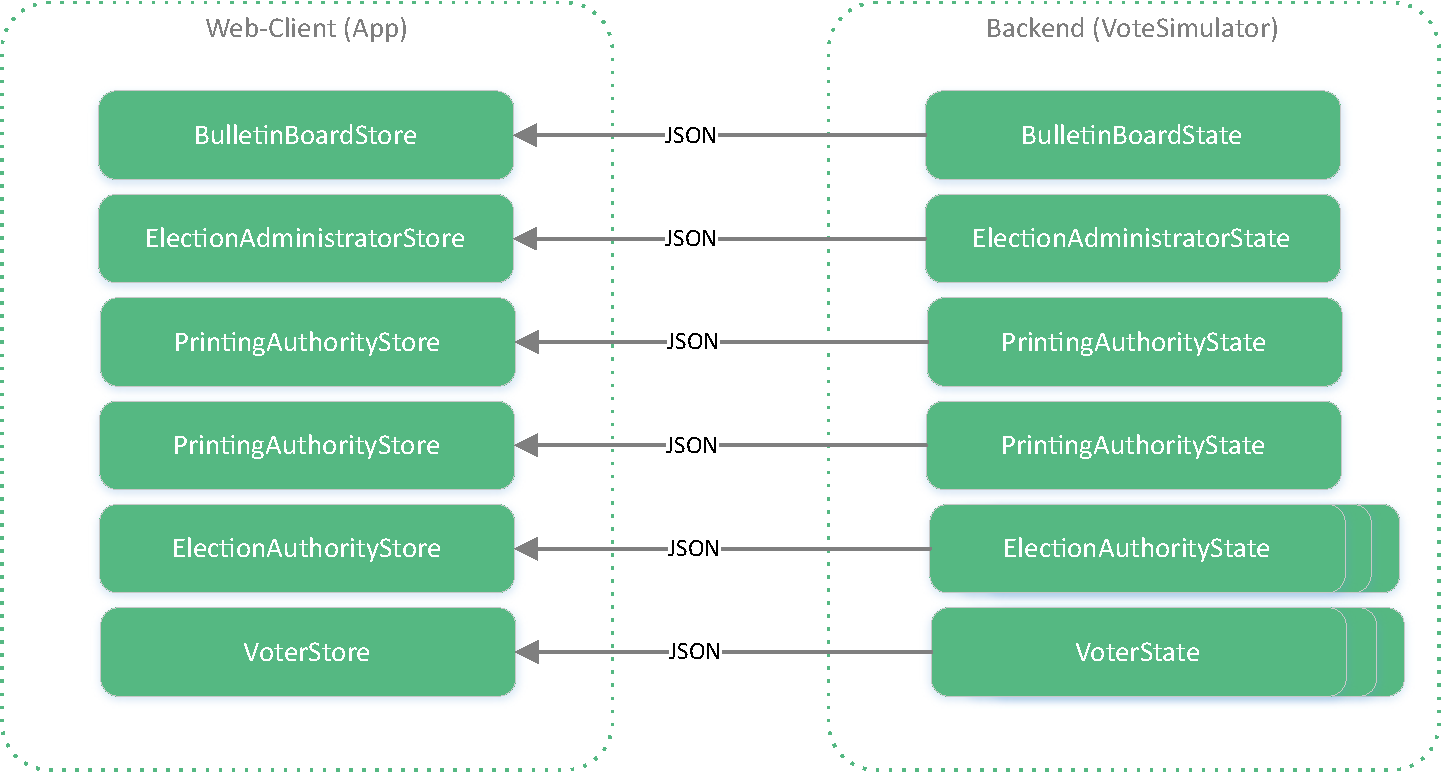
\includegraphics[scale=0.62]{assets/datastores.pdf}
\captionof{figure}{For every VoteService state, there is a corresponding datastore on the client side. The client side datastore are initially populated with the whole dataset during the initial loading procedure of an election event.}\label{Datastores}%
\end{center}
\end{figure}
After a client has populated his local data store, future manipulations on the backend are synchronized using the so called JSON Patch operations, which only contain the delta between the previous and the current state.

JSON Patch is a data structure for describing how a to patch / modify a JSON object. The procedure is standardized and described in the RFC 6902 of the Internet Engineering Task Force (IETF). There exist JSON Patch implementations for many languages, including Python and JavaScript. We used JSON Patch to realize our incremental data synchronization as follows:

When the VoteService loads the state of its actor objects, it sets the \mintinline{python}/originalState/ property of the actor to a deep copy of his state object. Mutations are always done only to the \mintinline{python}/state/ property. Before calling the \mintinline{python}/persist()/ method on an actor object, we use the Python JSON Patch library for determining the differences between the state and the originalState, to find out if and what variables have changed within the states. As a result, we receive a set of JSON Patch operations that describe how the \mintinline{python}/originalState/ could be patched, such that it becomes identical to the manipulated \mintinline{python}/state/ object, by calling 
\\ \mintinline{python}/make_patch(json.loads(self.originalState.toJSON()), json.loads(self.state.toJSON()))/

The result is an array of operations in JSON format that contains:
\begin{itemize}
	\item The path of the manipulation
	\item The type of operation (replace, add, remove, ...)
	\item The new value (if required)
\end{itemize}

For example: After casting a ballot, we might receive the following JSON patch:

\begin{figure}
\begin{center}
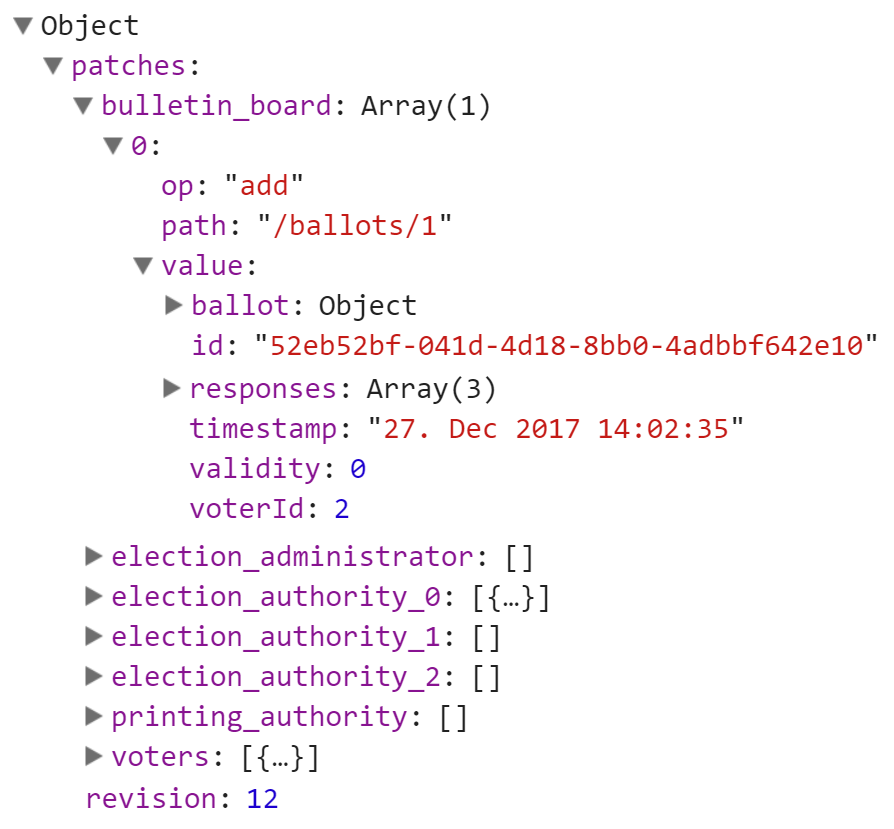
\includegraphics[scale=0.6]{assets/jsonpatchexample.png}
\captionof{figure}{JSON patch is an RFC standard that describes a procedure to incrementally patch a JSON object. By comparing two JSON objects JSON patch creates a set of operations that are needed to patch one object to match the other. We used JSON patch to keep the client side datastores in sync with the central database. The picture shows the resulting operations after submitting a new ballot.}\label{JSON Patch example}%
\end{center}
\end{figure}
These JSON patches are pushed to all the clients that need to receive the mutations and are applied to the local data-store which (under normal circumstances) contains the original state. After applying the JSON patch, the data store of all clients contains the same state of an election event as the back-end.

\begin{figure}
\begin{center}
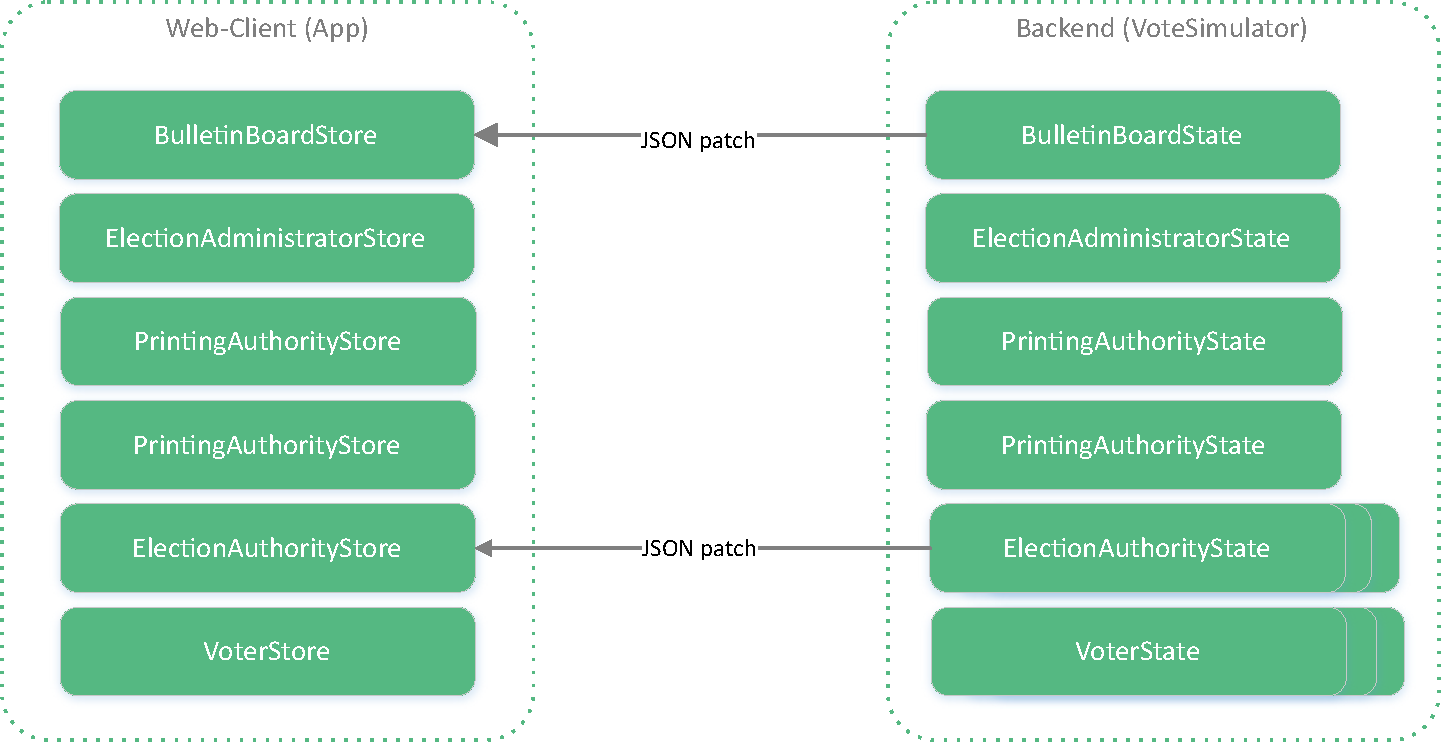
\includegraphics[scale=0.62]{assets/DatastoresJsonPatch.pdf}
\captionof{figure}{After the client side datastores have been initially loaded, future mutations of the central database are synchronized to all clients by receiving and applying JSON patches, which contain operations to patch the local data stores to be in sync with the back-end.}\label{Data-Sync with JSON Patches}%
\end{center}
\end{figure}

If for some reason, a web-client does not receive a JSON patch, its local data-store will no longer correspond to the back-ends version. This might happen because of network issues and an interrupted WebSocket connection or if applying the JSON patch operations failed.

For this reason we have invented a data-store revision-number for every election event, which is incremented whenever some state is manipulated and persisted on the back-end. This revision number is sent alongside the JSON patches to the clients, and is also stored on the client side. Before applying the JSON patches, the client checks if his local data-stores revision number is exactly 1 version behind the servers data store revision, which normally will be the case. If the client detects that his revision number is 2 or more versions behind the servers, it will request a full-data synchronization over the DataSyncService to avoid out-dated, corrupted local data stores.

During development, we ran into an issue with the python JSON patch library "`python-json-patch v1.16"' that we have been using. During some special cases the generation of JSON patches failed and resulted in an exception when comparing objects where mutations have been made to arrays within dictionaries - a combination which often occurs in our data structures. After hours of debugging and analyzing the issue, we have figured out a temporary workaround and reported the issue \footnote{https://github.com/stefankoegl/python-json-patch/issues/74} to the repository of the developers of this library. A few days later a new version v1.20 of the library had been released which fixed our issue.

\subsection{REST API}
The third component of the back-end is the REST API. Its responsibilities are to provide all the functionality of the VoteService to the web clients and trigger the data synchronization of the DataSyncService. Every function required by the front-end, such as \mintinline{python}/castVote()/ has a corresponding endpoint in the REST API service.

\begin{minted}[frame=single,framesep=10pt,tabsize=2,breaklines]{python}
@main.route('/castVote', methods=['POST'])
@cross_origin(origin='*')
def castVote():
    data = request.json
    electionId = data["election"]
    selection = data["selection"]
    voterId = data["voterId"]
    votingCode = data["votingCode"]

    if len(selection) == 0:
        return make_error(400, "Empty selection")

    try:
        svc = VoteService(electionId) # prepare VoteService

        svc.castVote(voterId, selection, votingCode) # perform vote casting

        patches = svc.persist()	# persist modified state and retrieve JSON patches

        syncPatches(electionId, SyncType.ROOM, patches)	# send the JSON patches to all clients

    except Exception as ex:
        return make_error(500, str(ex))

    return json.dumps({'result': 'success'})
\end{minted}

The API can be reached by sending a HTTP(S) POST request to our web server hosting the back-end services. The URL defines what function will be executed. For example: A POST request to https://<server>:5000/castVote/ would call the above function. The required parameters are provided in the POST body.

As a first step, parameters are extracted from the POST request and validated if necessary. As the next step, a VoteService object is instantiated by passing the electionId to the constructor. The VoteService will internally load the states of the corresponding election event from the database and instantiate the actor objects such as the election authorities.

Now the VoteService can execute the function which the user intended to call, for example "`CastVote"'. By calling the function \mintinline{python}/persist()/, the new state is written to the database and the JSON Patches of all mutations that "`CastVote"' has been made are determined, returned and can be sent to all clients by the help of the DataSyncService.

The following sequence diagram shows how the vote casting use case is implemented within the back-end and how all the components work together.

\begin{center}
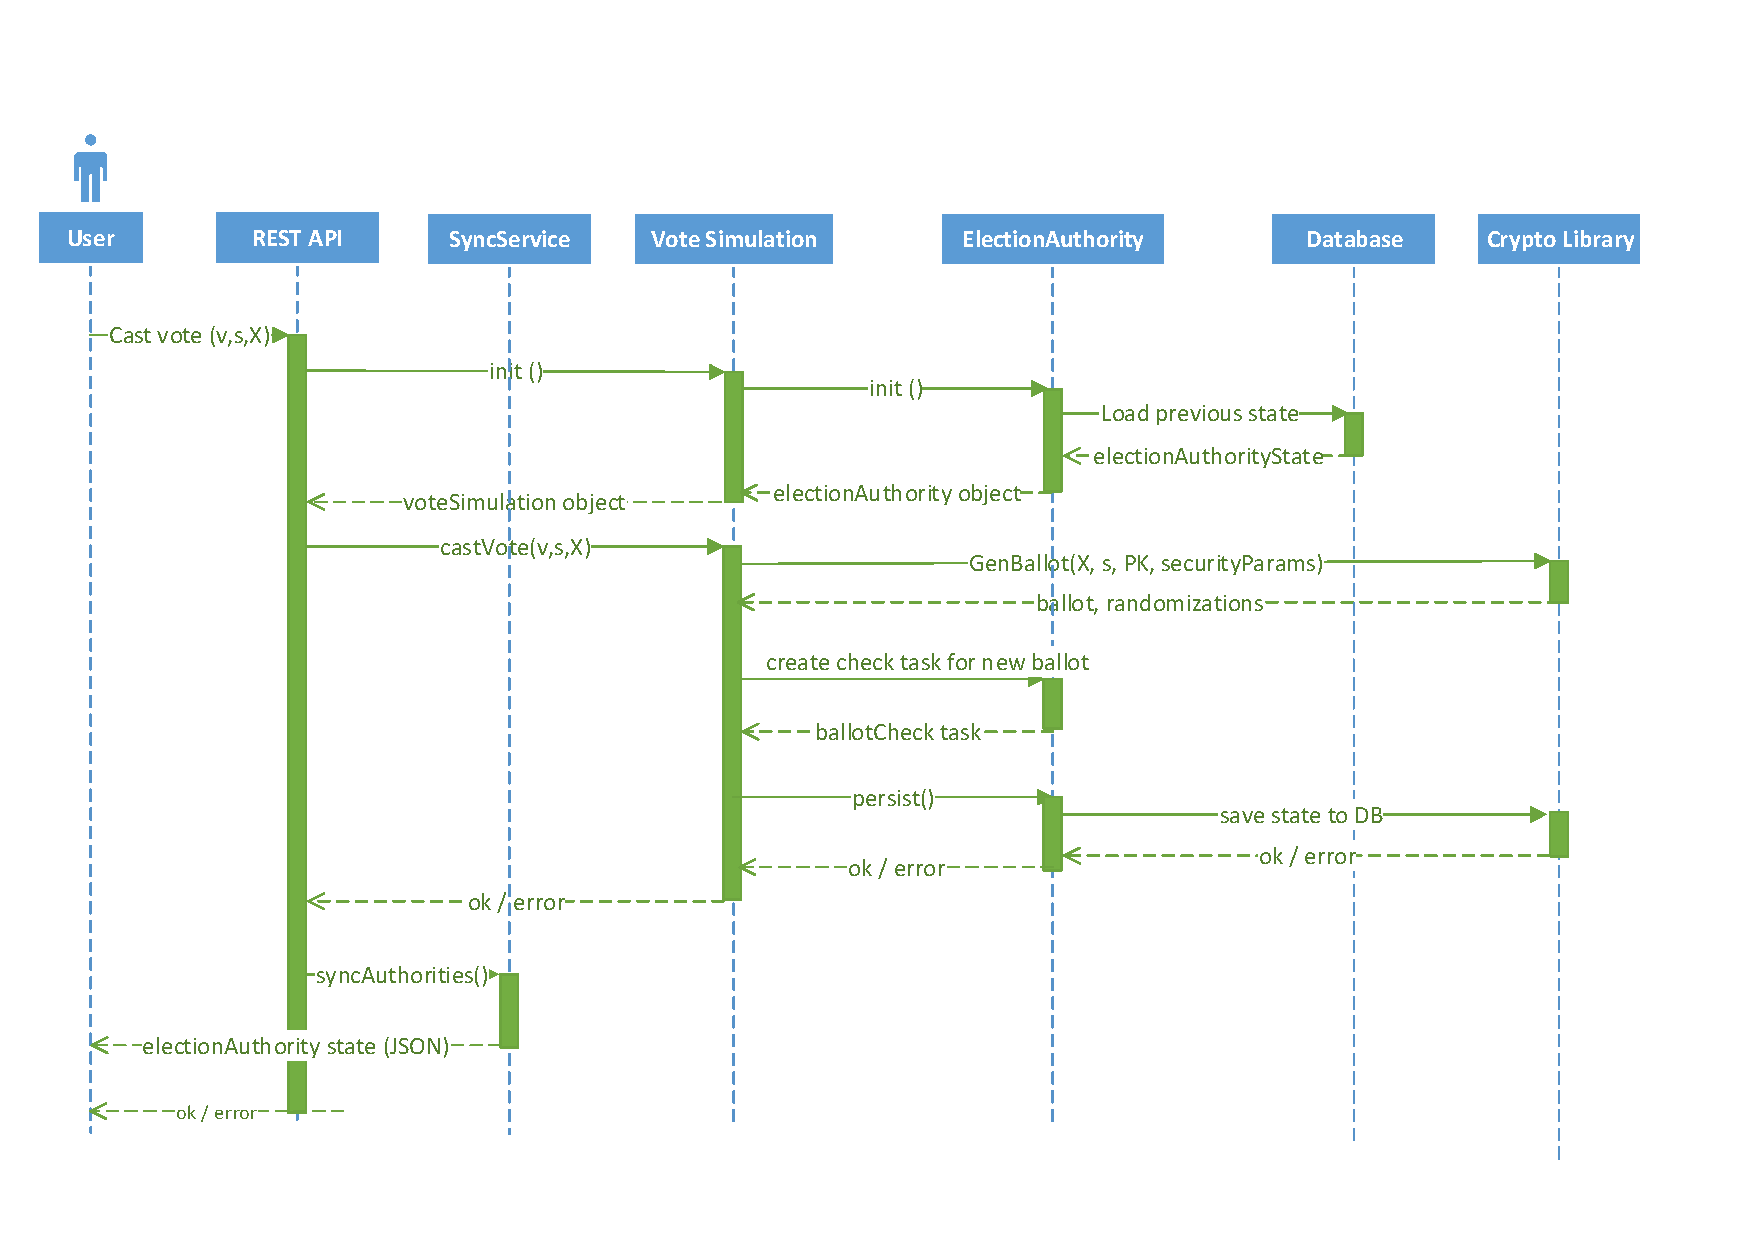
\includegraphics[scale=0.62]{assets/votecastingDiagram.pdf}
\captionof{figure}{Vote casting sequence diagram}\label{Vote casting sequence diagram}%
\end{center}

\section{Crypto-Library}

\subsection{File structure}
We decided to put every algorithm of the specification in its own file together with related unit tests. The files are structured according to the actors of the protocol, for example:

\begin{itemize}
	\item \textbf{Common}: contains common cryptographic algorithms and the security parameters used by multiple algorithms
	\item \textbf{ElectionAuthority}: contains all the algorithms used by the election authority
	\item \textbf{PrintingAuthority}: contains all the algorithms used by the printing authority
	\item \textbf{VotingClient}: contains all the algorithms used by the voting client
	\item \textbf{ElectionAdministration}: contains all the algorithms used by the election administrator
	\item \textbf{Utils}: contains helper classes and miscellaneous utility functions
\end{itemize}

\subsection{Public Parameters}
There exist two types of public parameters:

The \textbf{security relevant parameters}, e.g:

\begin{itemize}
	\item The order of the prime groups: $p$, $\prime{p}$, $\hat{p}$
	\item The length of the voting, confirmation, verification and finalization codes
	\item The number of authorities: $s$
\end{itemize}

and \textbf{public election parameters}, e.g.:

\begin{itemize}
	\item The size of the electorate: $N_E$
	\item The number of candidates: $n$
	\item The list of candidate descriptions: $c$
\end{itemize}

The security parameters are typically used within the algorithms and remain unchanged for a longer time period, whereas the public election parameters are different for every election event.

The object \texttt{SecurityParams} holds all security relevant parameters and is injected as an additional function argument to all algorithms. Several different \texttt{SecurityParams} objects are created initially, which contain all the parameters according to the recommendations in the CHVote specification document ("level 0" for testing purposes and "level 1" through "level 3" for productive use). For simple unit and debugging purposes, we can inject the "level 0" object while in production, level 1 - 3 are used.

The public election parameters on the other hand are directly passed to the algorithms by the calling party. If an algorithm needs to know certain election parameters (like the size of the electorate $N_E$), these values are typically derived from vectors that they have access to, so they do not require specific knowledge of these parameters.

\subsection{Coding Style}
The following source code sample shows a typical implementation of an algorithm (in this example, algorithm 7.18 according to the CHVote specification).

\begin{minted}[frame=single,framesep=10pt,tabsize=2,breaklines]{python}
import gmpy2
from Utils.Utils                    import *
from Crypto.SecurityParams          import *
from VotingClient.GetSelectedPrimes import GetSelectedPrimes
from VotingClient.GenQuery          import GenQuery
from VotingClient.GenBallotProof    import GenBallotProof
from Types                          import Ballot

def GenBallot(X_bold, s, pk, secparams):
    """
    Algorithm 7.18: Generates a ballot based on the selection s and the voting code X. The
    ballot includes an OT query a and a proof pi. The algorithm also returns the random
    values used to generate the OT query. These random values are required in Alg. 7.27
    to derive the transferred messages from the OT response, generated by Alg. 7.25.

    Args:
        X_bold (str):                   Voting Code X ∈ A_X^l_X
        s (list of int):                Selection s = (s_1, ... , s_k)
        pk (mpz):                       ElGamal key pk ∈ G_p \ {1}
        secparams (SecurityParams):     Collection of public security parameters

    Returns:
        tuple:                          alpha = (r, Ballot) = (r, (x_hat, a, b, pi))
    """
    AssertMpz(pk)
    AssertList(s)
    AssertClass(secparams, SecurityParams)

    x = mpz(StringToInteger(X_bold, secparams.A_X))
    x_hat = gmpy2.powmod(secparams.g_hat, x, secparams.p_hat)

    q_bold = GetSelectedPrimes(s, secparams)                    # q = (q_1, ... , q_k)
    m = mpz(1)

    for i in range(len(q_bold)):
        m = m * q_bold[i]

    if m >= secparams.p:
        return None

    (a_bold, r_bold) = GenQuery(q_bold, pk, secparams)
    a = mpz(1)
    r = mpz(0)

    for i in range(len(a_bold)):
        a = (a * a_bold[i]) % secparams.p
        r = (r + r_bold[i]) % secparams.q

    b = gmpy2.powmod(secparams.g,r, secparams.p)
    pi = GenBallotProof(x,m,r,x_hat,a,b,pk, secparams)
    alpha = Ballot(x_hat,a_bold,b,pi)

    return (alpha, r_bold)

class GenBallotTest(unittest.TestCase):
    def testGenBallot(self):
        selection = [1,4]       # select candidates with indices 1,4
        (ballot, r) = GenBallot(unittestparams.X, selection, unittestparams.pk, secparams_l0)
        print(ballot)
        print(r)

if __name__ == '__main__':
    unittest.main()
\end{minted}

All algorithms contain a short description, which was taken as-is from the specification document, as well as a comment (Google-style documentation string), which can be used to automatically generate code documentation. The algorithm itself is implemented as close to the specification as possible, using the same variable names and (as far as the language supports it) similar control structures:

\begin{itemize}
	\item The suffix \texttt{\_bold} for emphasized (bold) variables, e.g. \texttt{p\_bold} for \textbf{p}
	\item The suffix \texttt{\_hat} for variables with a hat, e.g. \texttt{a\_hat} for $\hat{a}$
	\item The suffix \texttt{\_prime} for variables with a prime, e.g. \texttt{a\_prime} for $a'$
	\item etc.
\end{itemize}

Each file also contains unit tests of the specific algorithm (if unit testing was considered useful for the particular algorithm).

The following example shows the similarities between the algorithm pseudo code and the actual implementation in Python:

\begin{multicols}{2}
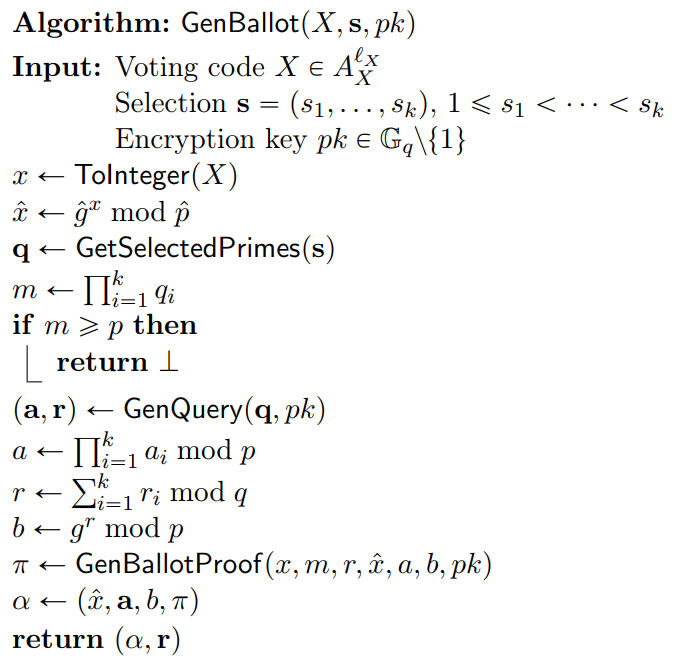
\includegraphics[width=0.46\textwidth]{assets/genballot.png}
\columnbreak
\begin{minted}[fontsize=\scriptsize]{python}
x = mpz(StringToInteger(X_bold, secparams.A_X))
x_hat = gmpy2.powmod(secparams.g_hat, x, secparams.p_hat)
q_bold = GetSelectedPrimes(s, secparams)

m = mpz(1)
for i in range(len(q_bold)):
    m = m * q_bold[i]

if m >= secparams.p:
    return None

(a_bold, r_bold) = GenQuery(q_bold, pk, secparams)
a = mpz(1)
r = mpz(0)

for i in range(len(a_bold)):
    a = (a * a_bold[i]) % secparams.p
    r = (r + r_bold[i]) % secparams.q

b = gmpy2.powmod(secparams.g,r, secparams.p)
pi = GenBallotProof(x,m,r,x_hat,a,b,pk, secparams)
alpha = Ballot(x_hat,a_bold,b,pi)

return (alpha, r_bold)
\end{minted}
\end{multicols}

\subsection{Return Types}
In most cases, when an algorithm returns more than a scalar datatype, tuples are used. Tuples allow to return multiple values from a function:

\begin{minted}[frame=single,framesep=10pt,tabsize=2,breaklines]{python}
def foo():
   return (1, 2)

def main():
   a, b = foo()
\end{minted}

This way large parts of the source code looked very similar to the pseudo code in the CHVote specification. For more complex data types or return values that are used more than once, named tuples were used. The data type "namedtuple" is like a lightweight class and allows access to named properties.

\begin{minted}[frame=single,framesep=10pt,tabsize=2,breaklines]{python}
Ballot = namedtuple("Ballot", "x_hat, a_bold, b, pi")

def main():
   Ballot b = getBallot()
   x_hat = b.x_hat
\end{minted}

By following this approach we could avoid having lots of container classes only used to pass data structures between the algorithms.

\section{Front-End}
The front-end was the most important component for our project, since we put focus mostly on the visualization and less on the actual e-voting system. Displaying the rather large amount of voting specific data and large numbers (>= 1024 bit) required a clean and well structured layout and a modular component design. Luckily, the framework we had chosen, VueJS, did very well in supporting us to meet exactly those requirements. We tried to follow the design patterns and best practices proposed by the makers of VueJS wherever possible.

In this section we will explain what concepts of VueJS we used and how we adapted them to our needs.

\subsection{Components}
Components are the basic building blocks of the VueJS framework. The application itself is a component, every page of the application is a component and the pages typically contain lots of components, one for every control like form controls, buttons or custom controls such as the ballot-list etc. The concept of components encourages to create reusable modules, provides a way to structure the application into smaller units and makes the resulting HTML template more expressive and easier to read.

We have created our own VueJS components for every control that we used more than once. For example the ballot list that is shown both in the bulletin board view as well as in the election authority view, the labels for displaying truncated large numbers or the cards used as our standard mean for displaying data have all been turned into custom components. One of the beautiful features of VueJS components is the concept of slots. By defining one or multiple slots within a components template markup, it becomes possible from the parent of a component, to embed content into different locations (slots) within the components HTML template.

We have been using slots to create our card component, which can display information either as the main content of the card, or within an expandable area on the bottom of the card:

\begin{minted}[frame=single,framesep=10pt,tabsize=2,breaklines]{javascript}
<DataCard title="Foo" :expandable=true>
		Just some text
		<p slot="expandContent">More complex content <BigIntLabel :mpzValue="publicKey"></BigIntLabel>
		</p>
</DataCard>
\end{minted}
The first line "`Just some text"', which gets inserted into the default unnamed slot, could as well be passed as a string parameter to the data card component. However, as things are getting more complicated, one might like to place arbitrary HTML or even another VueJS component inside the expandable content of our datacard. In such cases, component parameters will not work as they only accept primitive data types. Slots on the other hand allow arbitrary content to be injected.
\begin{figure}[h!]
\begin{center}
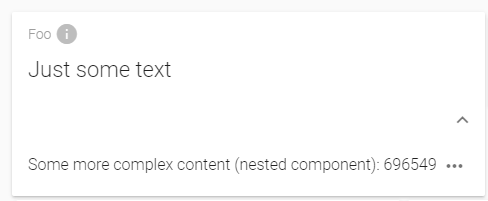
\includegraphics[scale=1.0]{assets/datacardexample.PNG}\\
\captionof{figure}{Our DataCard component that allows content to be injected in different places within its DOM by using the slot-concept of VueJS.}\label{DataCardXample}%
\end{center}
\end{figure}
The following code shows how the data-card component is implemented:

\begin{minted}[frame=single,framesep=10pt,tabsize=2,breaklines]{html}
<template>
    <v-card class="dataCard">
        <ConfidentialityChip v-if=showConfidentiality"' :type="confidentiality" class="confidentialityChip" />
        <v-card-title primary-title class="dataCardTitle">
            <div><span class="label grey--text">{{title}}
              <v-tooltip top>
                <v-icon v-if="!disableTooltip" color="grey lighten-1" slot="activator">info</v-icon><span>Programmatic tooltip</span>
             </v-tooltip></span>
            </div>
        </v-card-title>
        <v-card-text class="dataCardContent">
                <slot></slot>
        </v-card-text>
        <v-card-actions v-show="expandable">
            <v-btn icon @click.native="showExpander = !showExpander">
                <v-icon>{{ !showExpander ? 'keyboard_arrow_down' : 'keyboard_arrow_up' }}</v-icon>
            </v-btn>
        </v-card-actions>
        <v-slide-y-transition v-show="expandable">
            <v-card-text v-show="showExpander">
                <slot name="expandContent">
                </slot>
            </v-card-text>
        </v-slide-y-transition>
    </v-card>
</template>
<script>
    import { mapState } from 'vuex'

    export default {
      data: function () {
        return {
          showExpander: false
        }
      },
      computed: {
        ...mapState({
          showConfidentiality: state => state.showConfidentiality
        })
      },
      props: {
        title: {
          type: String,
          required: true,
          default: 'Title'
        },
        expandable: {
          type: Boolean,
          required: true,
          default: false
        },
        confidentiality: {
          type: String,
          required: true,
          default: 'public'
        },
        disableTooltip: {
          type: Boolean,
          required: false,
          default: false
        }

      },

      mounted () {
      }
    }
</script>
\end{minted}
The first part within the \mintinline{javascript}/<template>/ tag describes the HTML markup as well as the slots that we have just mentioned.

The \mintinline{javascript}/<script>/ tag contains the actual logic of the component, similarly to the controller in other SPA frameworks. The \mintinline{javascript}/data/ object contains variables which are defined and valid only locally within the component.  The \mintinline{javascript}/computed/ object maps variables from our central data-store to a local variable which is reactively bound to the data-store. Whenever the value of the given variable changes in the data-store, the computed property is automatically updated. From the template, we can access both local data as well as computed properties. Computed properties can also be used whenever a local variable needs to be formatted, or in some way manipulated before it is displayed in the components template.

The third source of data are properties (`props`), which are passed as arguments from the parent component. They are typically used to define options for a component.

Additionally, components may contain \mintinline{javascript}/methods/, typically used for event-handlers like button clicks and event hooks like \mintinline{javascript}/mounted/, \mintinline{javascript}/beforeDestroy/, \mintinline{javascript}/beforeCreated/ to influence the components creation/destruction at different times during a components lifecycle.

\subsection{Centralized Data-Store \& Flux Pattern}
One of the big challenges regarding the architecture of our front-end, was about how and where we would store all the data of an election. Clearly, since we already had divided an election events data into one state for every actor and given that every actor also has its corresponding view in our front-end, simply storing the data to the respective component has been our first thought. Although a voter mainly needs to access his own data contained in the voters state, some data must be shared between multiple components, for example the information on the bulletin board.

Since we wanted to avoid having to keep data redundant in multiple components, we have decided to use the Flux design pattern in our front-end. The basic idea of the flux pattern is to have a single, central data source where all the data is stored and which all components have access to. This single data source is called a "`store"' by Flux terminology. VueJS has its own implementation of the Flux pattern called \textit{Vuex}. Another important concept is that components can freely access the data in the store, however, they are not allowed to change data, at least not directly. Instead, if a component wants to manipulate data in the store, this has to be done by calling \textbf{mutation functions}. Not allowing direct manipulation of the store makes it much easier to keep track of where mutations came from.

Our web applications data store is divided into multiple modules, one data store module for each corresponding state of the back-end. In reality, all these data stores are part of one single data store, but having multiple modules allows us to structure the mutation and getter functions and help to avoid naming conflicts by having separate namespaces for every module.

The data-store can be accessed from any component by defining a computed property. If the computed properties have to perform some formatting, aggregation, filtering etc. on the state variables and are used from within multiple components, it is also possible and recommended to write getter-functions in the data-store to avoid redundancy.

\subsection{Internationalization (i18n)}

All text visible to the user on the front-end of the application is internationalized, i.e. the display language can be changed at any time by the user. The default language provided is English and translations for German have been added. The main language, English, and the manual translations for German are stored in the translations preset YAML file \texttt{frontend/src/translations.preset.yaml}. By using the translation script \texttt{frontend/src/translate.js}, those languages stored in the preset file can be translated automatically to predefined target languages. Those automatic translations (provided via Google Translate) are stored together in the YAML file \texttt{frontend/src/translations.yaml} together with the main language and manual translations. This file is used to provide translations for the front-end application. 

% TODO

\subsection{Development Environment}
During development Webpack is used. Webpack is a module bundler, i.e. a piece of software which generates static assets from JavaScript libraries including all dependencies, CSS files, images etc. Additionally, webpack features a development web server, which aids in fast development. While the development server is running, any changes in the application's source code are detected and assets are re-generated on the fly. This way, any changes in the application are directly visible in the browser.

% TODO

\subsection{Staging Environment}
In order to deploy the application to an environment for staging purposes, we have decided to use Docker together with Docker Compose. The Docker Compose file \texttt{docker-compose.yaml} stores the configuration for three distinct Docker containers: a MongoDB service, the back-end and the front-end. By running \texttt{docker-compose build} in the project's root directory, those three containers can be built. After building the containers, the services can be started by running \texttt{docker-compose up}. The application will then be available via \texttt{localhost:8080} (TCP).

\section{Challenges}
In this section we describe some of the challenges that we encountered while developing our application.

\subsection{WebSocket subscription concept}
Since our application allows that multiple election events exist at the same time, the question arose how we could handle that only those clients who are actually observing a particular election event receive web-socket messages when an action has been triggered on the back-end and concerning the particular election event.

We have seen similarities between our problem and the one a typical chat has that consists of multiple chat-rooms in which only those users should be notified of new posts that have actually joined the room. We have adapted this "`chat-room"' concept to our problem by defining a room to be equal to an election event.

We can assume that all the pages that actually show data of an election evemt require the election events id to be passed as part of the URL. For example: /BulletinBoard/1 is the route to reach the BulletinBoard view of the election with id 1.

Whenever a route is called that contains the argument `electionId`, we need to make sure that the client has joined the room of this election event. We therefore set a global variable called \mintinline{python}/joinedElectionId/ to match the id of the election event a user has joined. We created a VueJS "`mixin"' that can be added to every election page, which makes sure that if the client has not yet joined the corresponding election events room, it emits a "`join"' request to the socket.io server, passing along the electionId:

\begin{minted}[frame=single,framesep=10pt,tabsize=2,breaklines]{javascript}
export default {
  created () {
    if (this.$store.getters.joinedElectionId !== this.$route.params.electionId) {
      this.$socket.emit('join', {election: this.$route.params['electionId']})
    }
  }
}
\end{minted}
On the server side, we have defined a socket.io listener called "`join"' which will remove the calling client from every room before joining the room of the requested election event. There is only one exception: The client cannot leave the room that corresponds to the `sid` of the request, since this is basically the channel over which the `join` request is handled.
\begin{minted}[frame=single,framesep=10pt,tabsize=2,breaklines]{python}
@socketio.on('join')
def on_join(data):
    electionID = data['election']
    for room in rooms():
        if room != request.sid:																	# do not leave the room of the current connection
            leave_room(room)
    join_room(electionID)

    syncService.fullSync(electionID, SyncType.SENDER_ONLY)			# Perform a full data-sync

    emitToClient('joinAck', electionID, SyncType.SENDER_ONLY)		# send an acknowledgement/confirmation to the client
\end{minted}

The \mintinline{javascript}/joinAck/ handler in the web application will then set the \mintinline{javascript}/joinedElectionId/ variable to the just joined election id, such that the join will only be called once or until the user chooses a different election.

\subsection{Python issues} \label{ssec:PythonIssues}

During the project we have experienced a few issues with Python as the programming language that we used to implement the crypto-library and the back-end. In particular, we have observed the following issues:

\begin{itemize}
	\item Performance issues due to Python being an interpreted language
	\item Function overhead: function calls in Python seem to be very slow, especially when using recursions (such as recHash)
	\item Strongly dynamic typing vs. static typing: the Python interpreter needs to inspect every single object during run time (be it an integer or a more complex object)
	\item The \textit{BigInteger} library surprisingly is not as fast as using directly the GMP library, and using the GMP bindings also means that there is an overhead compared to a native BigIntegers.
\end{itemize}
As performance was not the main focus of our application, these issues were mostly ignored.

The following issues were more problematic for our project:
\begin{itemize}
	\item Because of the dynamic typing, the code becomes much more error-prone, as there is no standard checking of function argument types etc. We have tried to overcome this issue by using asserts to check the types of input parameters very often.
	\item There are little to no standards regarding the project structure when using our "`crypto-library"' approach. Most solutions depend on pathes set as environment variables or absolute imports, which we wanted to avoid. We have chosen to use relative imports and define the crypto-library as a module, which explains why there are many empty "`\_\_init\_\_.py"' files in our solution, which are required for this module-approach.
\end{itemize}

For detailed information regarding the performance issues that we have experienced see \cite{slowpy} and \cite{slowpy2}. Based on the reasons above we would not recommend to use Python for the use in similar or larger projects. Python is indeed a very handy language to write quick prototypes and proof of concepts, but issues become more frequent in larger projects.

\section{Automatic Task Processing for Election Authorities}
In our application, every election authority normally has to manually process all incoming tasks such as ballot checking, confirmation checking, mixing and decrypting. As it can become cumbersome to repeat the same steps multiple times during a short presentation, it might be desirable to perform these tasks manually only for the first election authority. Because of that we have implemented an automatic-mode in which an election authority automatically performs all tasks.

There were several different ways how we could have implemented this feature. One possibility would have been building a service which runs in the background and regularly checks for new tasks and processes them. Since every task requires a preceding action (for example: A Ballot-Check-Task requires a voter casting a vote), and since it is reasonable for our use-cases to assume that the authorities perform the tasks sequentially, we have chosen the most simple approach:

When a user casts a ballot and a ballot-check-task is created, we check if the first authority is set to automatic. If yes, the function for checking this ballot is automatically called for the first election authority. This function again checks, if the next election authority is set to automatic and recursively calls itself if that is the case, and so on until one authority has is called that is not set to automatically process the tasks.

This means that if the first authority is in manual mode and the other two are set to automatic, they both wait with their execution until the first election authority has manually started executing the task. This strict sequential order is only required by the protocol for the mixing task, all other tasks could be called in any order. If desired, this behavior could also be implemented with our approach, by simply executing the function for every authority with auto-mode set to true.

\section{Testing}
We have applied different testing concepts for the several components of our application.

The front-end has been tested using manual test-cases. One of the test-cases is shown as follows, the others can be found in the appendix. We have decided not to use automatic end-to-end or unit testing on our front-end because this would have generated a lot of work both for learning and integrating the testing frameworks like karma and selenium, and for writing the actual tests.

\begin{testcase}{Pre-Election}
	\addrow{Test-Case}{1. Pre-Election}
	\addrow{Description}{This test covers all the pre-election steps, including the creation of a new election, setting it up from the election administration view and the printing- and delivery of the voting cards}
	\addrow{Precondition}{ }
	\addrow{Postcondition}{
		\begin{itemize}
			\item The election event is in the status "`Election"'
			\item The voters have received a voting card
		\end{itemize}
	}
	\addstepsrow{Steps}{
	        \item Start our application
		\item Choose \textbf{Election Events} from the main menu
		\item Click on \textbf{\textit{Create new election event}}
		\item Enter a name for the election event and choose a security level and click on \textbf{\textit{create}}
		\item The \textbf{Election Admin} tab should now have an interaction notification
		\item Visit the \textbf{Election Admin} view
		\item Enter at least 3 for the number of voters, at least 3 different candidates and 1 for the number of selection and click on \textbf{\textit{Setup Election Event}}
		\item The \textbf{Printing Authority} tab should now have an interaction notification
		\item Visit the \textbf{Printing Authority} view
		\item Click on \textbf{Print Voting Cards}
		\item The voting cards for all voters should now be displayed
		\item Click on \textbf{Deliver Voting Cards To Voters}
		\item The voting cards should now disappear and the \textbf{Voters} tab should now have an interaction notification
		\item Visit the Voters view, select a voter and check that the voting card is displayed correctly
	}
\end{testcase}

For our back-end, we have used automatic unit testing wherever it made sense, especially for the CHVote algorithms. Most basic algorithms that were used within other algorithms, such as hashing, prime number generation etc., have unit-tests provided within the same file. More complex algorithms are not tested with unit-tests, especially when they require input generated by other algorithms. Algorithms like genShuffleProof and checkShuffleProof are tested by our voteSimulation test. If a shuffleProof can be generated and is recognized as a valid proof by checkShuffleProof and passes all internal asserts, we assume that it is working properly.

Additionally, we have used asserts a lot in our backend to compensate for the missing of static typing of the Python programming language and to make sure that both the input as well as the output of the algorithms are correct in terms of boundaries, dimensions, etc.

\definecolor{vmcol}{RGB}{150,150,150}
\definecolor{nmcol}{RGB}{200,200,200}
\definecolor{zscol}{RGB}{83,142,213} % red: 217,151,149
\definecolor{zicol}{RGB}{194,214,154}

\newcommand{\zs}[0]{\cellcolor{zscol}}				% soll
\newcommand{\zi}[0]{\cellcolor{zicol}}				% ist
%\newcommand{\ms}[0]{\makebox[.613cm][r]{$\blacklozenge$}}	% Meilenstein
\newcommand{\ms}[1]{
	\makebox[.7cm][r]{
		\tikz[baseline=(char.base)]{
			\node[shape=circle,draw,inner sep=.02cm,fill=black,text=white] (char) { #1 };
		}
	}
}

\newcommand{\sq}[1]{\textcolor{#1}{\rule{.3cm}{.3cm}}}

\newcommand{\phase}[1]{
	\multicolumn{22}{l}{} \\
	\multicolumn{22}{l}{\cellcolor{gray!20}\textbf{#1}} \\ \hline
}

\begin{landscape}
\section{Time schedule}

\begin{table}[h]
\centering
\renewcommand{\arraystretch}{1.2}
\fontsize{2mm}{2mm}\selectfont
\begin{tabular}[c]{
	|m{7cm}|l
	*{10}{
		|>{\centering\arraybackslash}m{.3cm}
		|>{\centering\arraybackslash}m{.3cm}
	}
	|}

\hline

\textbf{Project tasks} & & 38 & 39 & 40 & 41 & 42 & 43 & 44 & 45 & 46 & 47 & 48 & 49 & 50 & 51 & 52 & 53 & 54 \\ \hline

\phase{Documentation}
\multirow{2}{*}{Update documentation and journal}
& soll & \zs & \zs & \zs & \zs & \zs & \zs & \zs & \zs & \zs & \zs & \zs & \zs & \zs & \zs & \zs & \zs & \zs \ms{5} \\ \hhline{~*{21}{-}}
& ist  & \zi & \zi & \zi & & & \zi & & \zi & \zi & & & & & & & & \\ \hline

\phase{Concept}
\multirow{2}{*}{Working out goals / requirements}
& soll & \zs & \zs & \zs & & & & & & & & & & & & & & \\ \hhline{~*{21}{-}}
& ist  & \zi & \zi & \zi & \zi & \zi & & & & & & & & & & & & \\ \hline
\multirow{2}{*}{Concept}
& soll & & \zs & \zs & & & & & & & & & & & & & & \\ \hhline{~*{21}{-}}
& ist  & & \zi & \zi & \zi & & & & & & & & & & & & & \\ \hline

\phase{Implementation}
\multirow{2}{*}{Update CHVote cryptolibrary to the lastest specification}
& soll & \zs & \zs\ms{1} & & & & & & & & & & & & & & & \\ \hhline{~*{21}{-}}
& ist  & \zi & \zi & & & & & & & & & & & & & & & \\ \hline
\multirow{2}{*}{Prototyping (proof of concept)}
& soll & & & \zs & \zs\ms{2} & & & & & & & & & & & & & \\ \hhline{~*{21}{-}}
& ist  & & & \zi & \zi & & & & & & & & & & & & & \\ \hline

\phase{Iteration 1}
\multirow{2}{*}{Implement backend API}
& soll & & & & & \zs & \zs & \zs & \zs & \zs & \zs & & & & & & & \\ \hhline{~*{21}{-}}
& ist  & & & & & \zi & \zi & \zi & \zi & \zi & & & & & & & & \\ \hline
\multirow{2}{*}{Implement frontend: Pre-election}
& soll & & & & & & & \zs & \zs & & & & & & & & & \\ \hhline{~*{21}{-}}
& ist  & & & & & & & \zi & \zi & & & & & & & & & \\ \hline
\multirow{2}{*}{Implement frontend: Election}
& soll & & & & & & & & \zs & \zs & & & & & & & & \\ \hhline{~*{21}{-}}
& ist  & & & & & & & & \zi & \zi & & & & & & & & \\ \hline
\multirow{2}{*}{Implement frontend: Post-election}
& soll & & & & & & & & & \zs & \zs\ms{3} & & & & & & & \\ \hhline{~*{21}{-}}
& ist  & & & & & & & & & \zi & & & & & & & & \\ \hline

\phase{Iteration 2}
\multirow{2}{*}{Automation of election authority (R19)}
& soll & & & & & & & & & & & \zs & & & & & & \\ \hhline{~*{21}{-}}
& ist  & & & & & & & & & & & & & & & & & \\ \hline
\multirow{2}{*}{Voting Card layout, Scratchcard (R15)}
& soll & & & & & & & & & & & \zs & \zs & & & & & \\ \hhline{~*{21}{-}}
& ist  & & & & & & & & & & & & & & & & & \\ \hline
\multirow{2}{*}{Election Overview (R8, R9)}
& soll & & & & & & & & & & & & \zs & \zs & & & & \\ \hhline{~*{21}{-}}
& ist  & & & & & & & & & & & & & & & & & \\ \hline
\multirow{2}{*}{k-out-of-n election types (R7)}
& soll & & & & & & & & & & & & & \zs & & & & \\ \hhline{~*{21}{-}}
& ist  & & & & & & & & & & & & & & & & & \\ \hline
\multirow{2}{*}{Improving the input forms and layout (R11)}
& soll & & & & & & & & & & & & & & \zs & & & \\ \hhline{~*{21}{-}}
& ist  & & & & & & & & & & & & & & & & & \\ \hline
\multirow{2}{*}{Variable security level (R13)}
& soll & & & & & & & & & & & & & & & \zs & & \\ \hhline{~*{21}{-}}
& ist  & & & & & & & & & & & & & & & & & \\ \hline
\multirow{2}{*}{Verifier functionality (R23) and reserve}
& soll & & & & & & & & & & & & & & & \zs & \zs\ms{4} &\\ \hhline{~*{21}{-}}
& ist  & & & & & & & & & & & & & & & & & \\ \hline
\phase{Project completion}
\multirow{2}{*}{Poster, Final Day, Presentation}
& soll & & & & & & & & & & & & & & & & \zs & \zs \\ \hhline{~*{21}{-}}
& ist  & & & & & & & & & & & & & & & & & \\ \hline

\end{tabular}
\caption{Project time schedule}
\end{table}

\end{landscape}

\chapter{Journal}

\section{Week 1}
\subsection{Reflexion}

During our kickoff meeting we discussed the several possibilities of our
bachelor thesis based on the spadework of the previous "project 2" module and
broke them down into two options: A realistic prototype of the whole chVote
system that includes everything a real implementation would need, like
signatures, channel security, distributed election authorities with docker
etc., or an interative prototype ("demonstrator") that allows to demonstrate
the functionality of the chVote protocol in a more visual manner.

\subsection{Next steps}

\section{Week 2}
\subsection{Reflexion}

The following week we have made the decision to build the demonstrator mainly
because the final product would potentially be more attractive visually than a
prototype where the main work is hidden behind the scences. We have also
started thinking about what technologies and frameworks to use and to build a
few sketches and mockups to have some basis for discussion for our next
meeting. At this stage we have yet been very unsure about how the application
should look like, what audience we should have as our main target and what
functionality the application should offer.

During our second meeting we ellaborated the goals and some more technical details.
\begin{itemize}
\item In essence, the application should allow to demonstrate a chVote election from the view of every party participating in the election process.
\item The system should manage multiple elections
\item The application should be a realtime webapp that updates the views automatically as soon as something changes and without having to reload the page
\end{itemize}

\subsection{Next steps}

\section{Week 4}
\subsection{Reflexion}

In the third week we finished describing the goals and further worked on the
system architecture. We also made some first experiences with the envisaged
frameworks and technologies (VueJS, socket.io, Flask, MongoDB).

\begin{itemize}
\item working with socket.io and VueJS has been very intuitive and looked very promising and suitable for our project
\item We were not yet sure whether or not mongoDB is the right technology for our needs.
\end{itemize}

\subsection{Next steps}

\chapter{Conclusion}

The future of e-voting in Switzerland is still unclear. With the efforts made
to publish the CHvote specification, finally a lot of issues involved with
e-voting have been solved. Unfortunately, an ordinary citizen does not have any
in-depth knowledge in cryptography in order to understand a protocol like
CHvote. So the introduction of a modern e-voting system in Switzerland or in
any other country in general depends on how strongly people believe and trust
such a protocol. This is were we hope that our application will help people to
understand how a modern e-voting system works. Although the protocol itself is
quite complicated, our application allows to explain and visualize the basic
ideas of modern e-voting.

\section{Reflection}

Vue.js turned out to be the perfect framework for coding the front-end of the
application. It allowed us to develop in small bits, always being able to
directly preview each step rendered in the browser. As for the back-end, we
still strongly believe that the choice of Python wasn't the correct one for
this kind of project. Python seems to be the number one choice for prototyping,
but for larger applications a lot of issues appear while developing.
Unfortunately, as we already implemented the CHvote protocol as part of
"Projekt 2" in Python, it did not make much sense to rewrite everything in a
different language, since it would have been too time consuming.



\begin{thebibliography}{999}
	\bibitem{chvote}
	"CHVote System Specification", by Rolf Haenni, Reto E. Koenig, Philipp Locher and Eric Dubuis, October 31, 2017, \url{https://eprint.iacr.org/2017/325}

	\bibitem{evotinganforderungen}
	"{}Anforderungskatalog für eidgenössische Volksabstimmungen mit der elektronischen Stimmabgabe"{}, by Bundeskanzlei BK, June 07.2014.

	\bibitem{aso}
	"{}ASO Factsheet E-Voting"{}, by Auslandschweizer-Organisation, \url{http://aso.ch/files/webcontent/direction/Factsheets/ASO_Factsheet_E-Voting.pdf}
	
	\bibitem{swissinfo}
	"{}Geneva mounts e-voting charm offensive"{}, by Swissinfo, \url{https://www.swissinfo.ch/eng/politics/pitching-for-partners_geneva-mounts-e-voting-charm-offensive/42439582}

	\bibitem{slowpy}
	"Why Python is Slow: Looking Under the Hood", by Jake VanderPlas, see \url{http://jakevdp.github.io/blog/2014/05/09/why-python-is-slow/}

	\bibitem{slowpy2}
	"Python speed: performance tips", from the official Python wiki, see \url{https://wiki.python.org/moin/PythonSpeed/PerformanceTips}
\end{thebibliography}


\end{document}
